% !TeX encoding = UTF-8
% !TeX program = xelatex
% !TeX spellcheck = en_US

\documentclass[degree=project,degree-type=project,cjk-font=noto]{thuthesis}
\usepackage{mathtools}
\usepackage{tikz}
\usetikzlibrary{shapes,arrows}
\usepackage[autosize]{dot2texi}
% Syntax Highlighting in LaTeX, need pygments
% Must build with xelatex -shell-escape -enable-8bit-chars.
\usepackage{minted}
% https://tex.stackexchange.com/a/112573
\usepackage{tcolorbox}
\usepackage{etoolbox}
\BeforeBeginEnvironment{minted}{\begin{tcolorbox}}%
\AfterEndEnvironment{minted}{\end{tcolorbox}}%
% color for minted
\definecolor{friendlybg}{HTML}{f0f0f0}


% 论文基本配置,加载宏包等全局配置
\thusetup{
    output = electronic,
    title  = {实验三:基于 PPG 的语音转换系统},
    author  = {肖文韬},
    studentid = {2020214245},
    course = {语音信号数字处理},
    include-spine = false,
}

\usepackage{float}
\usepackage[sort]{natbib}
\bibliographystyle{thuthesis-numeric}
\graphicspath{{figures/}}


\begin{document}

% 封面
\maketitle

\frontmatter
% % !TeX root = ../thuthesis-example.tex

% 中英文摘要和关键字

\begin{abstract}
  论文的摘要是对论文研究内容和成果的高度概括。摘要应对论文所研究的问题及其研究目
  的进行描述,对研究方法和过程进行简单介绍,对研究成果和所得结论进行概括。摘要应
  具有独立性和自明性,其内容应包含与论文全文同等量的主要信息。使读者即使不阅读全
  文,通过摘要就能了解论文的总体内容和主要成果。

  论文摘要的书写应力求精确、简明。切忌写成对论文书写内容进行提要的形式,尤其要避
  免“第 1 章……;第 2 章……;……”这种或类似的陈述方式。

  本文介绍清华大学论文模板 \thuthesis{} 的使用方法。本模板符合学校的本科、硕士、
  博士论文格式要求。

  本文的创新点主要有:
  \begin{itemize}
    \item 用例子来解释模板的使用方法;
    \item 用废话来填充无关紧要的部分;
    \item 一边学习摸索一边编写新代码。
  \end{itemize}

  关键词是为了文献标引工作、用以表示全文主要内容信息的单词或术语。关键词不超过 5
  个,每个关键词中间用分号分隔。(模板作者注:关键词分隔符不用考虑,模板会自动处
  理。英文关键词同理。)

  % 关键词用“英文逗号”分隔
  \thusetup{
    keywords = {TeX, LaTeX, CJK, 模板, 论文},
  }
\end{abstract}

\begin{abstract*}
  An abstract of a dissertation is a summary and extraction of research work
  and contributions. Included in an abstract should be description of research
  topic and research objective, brief introduction to methodology and research
  process, and summarization of conclusion and contributions of the
  research. An abstract should be characterized by independence and clarity and
  carry identical information with the dissertation. It should be such that the
  general idea and major contributions of the dissertation are conveyed without
  reading the dissertation.

  An abstract should be concise and to the point. It is a misunderstanding to
  make an abstract an outline of the dissertation and words ``the first
  chapter'', ``the second chapter'' and the like should be avoided in the
  abstract.

  Key words are terms used in a dissertation for indexing, reflecting core
  information of the dissertation. An abstract may contain a maximum of 5 key
  words, with semi-colons used in between to separate one another.

  \thusetup{
    keywords* = {TeX, LaTeX, CJK, template, thesis},
  }
\end{abstract*}


% 目录
\tableofcontents

% 插图和附表清单
\listoffigures           % 插图清单

% 正文部分
\mainmatter

\chapter{任务一: 提取 PPG 与声学参数 ($15"$)}

\section{任务介绍}

为了进行语音转换,我们首先需要使用 ASR 系统将源音频转换为一种中间特征(在本实验中就是音素序列 PPG~\cite{PPG}),对每一帧的 MFCC 特征 $X_t$ 我们可以得到所有音素(音素集 $\mathcal{S}$)的后验概率 $\{p(s | X_t) | s \in \mathcal{S}\}$。
同时,我们还可以将原始波形序列加窗得到语音帧,对语音帧进行离散傅里叶变换后,计算各频率分量的能量后可以得到语谱图(线性谱)。
而我们知道人类对低频成分更加敏感,而对高频不敏感,所以我们取对数后可以得到对应的 Mel 谱。
本任务就是使用预训练模型得到音频的 PPG,同时还需要计算得到基频 $F_0$, 线性谱,Mel 谱等声学参数。

接下来的小节就是回答问题啦。

\section{提取音素后验概率 PPG ($4"$)}

\textbf{(1) 简要说明 PPG 提取器(ppg\_extractor)的网络结构,给出网络的基本结构图。}

\begin{figure}[!htp]
\centering%
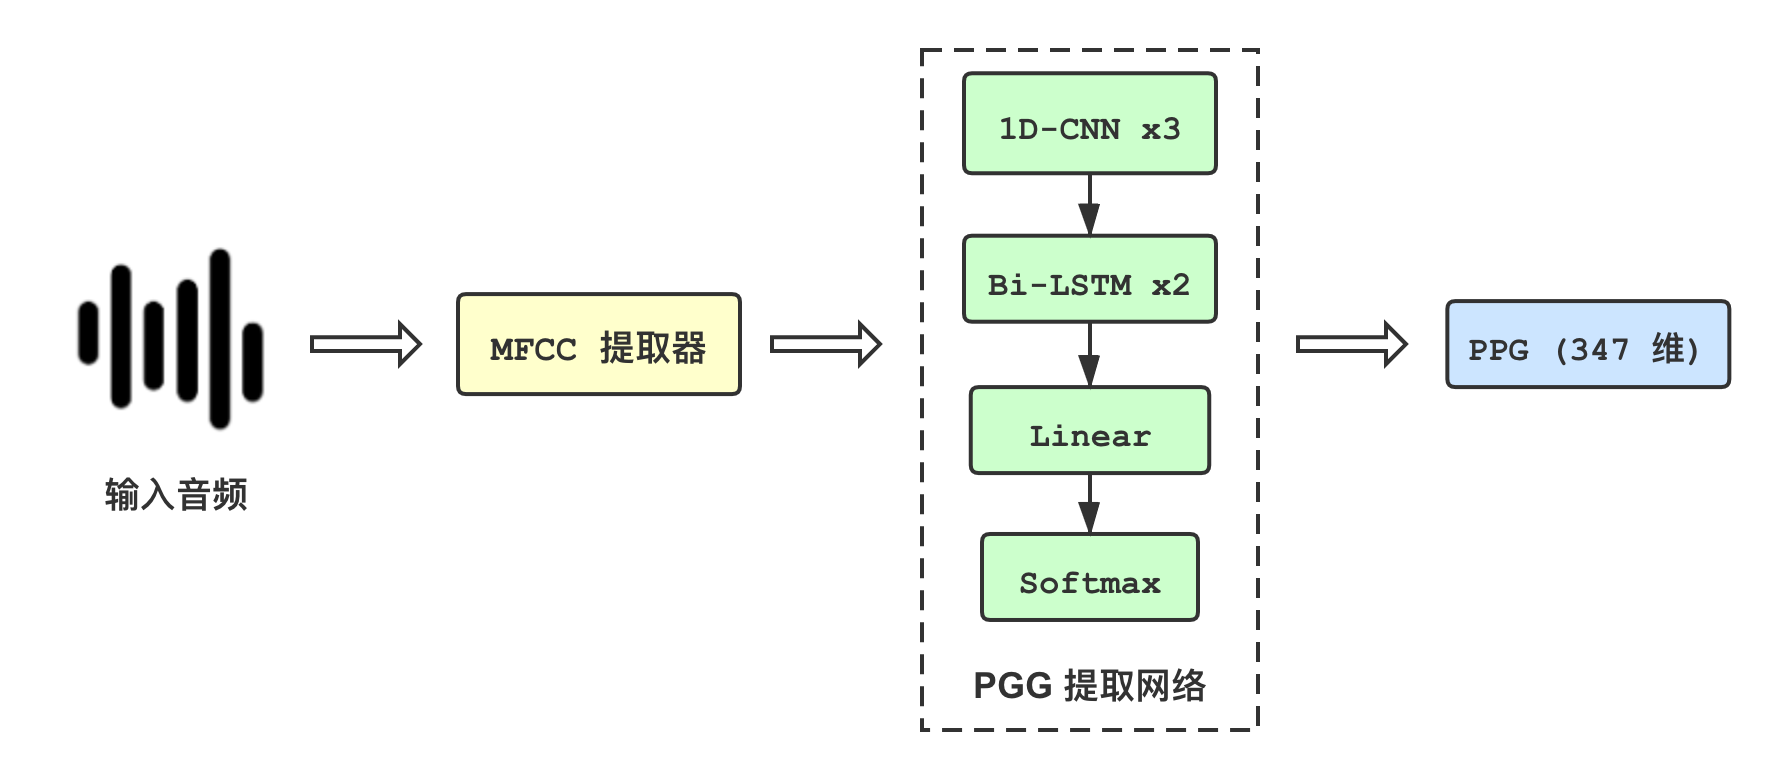
\includegraphics[width=.8\linewidth]{PPG.png}
  \caption{PPG 提取流程图}
  \label{fig:ppg}
\end{figure}


\textbf{答}: PPG 提取器网络由卷积层、LSTM 和线性层组成,具体组成如图~\ref{fig:ppg}所示。

\chapter{任务二: 训练并测试特定目标说话人的语音转换模型($40"$)}

\chapter{任务三: 探究残差网络对转换性能的影响($15"$)}

\chapter{任务四: 增加说话人嵌入网络,实现多目标说话人的语音转换($20"$)}

% 其他部分
\backmatter

% 参考文献
\bibliography{ref/refs}  % 参考文献使用 BibTeX 编译

% 附录
\appendix
\end{document}
